\documentclass{beamer}
%Information to be included in the title page:
\usetheme{Boadilla}
\definecolor{MITRed}{RGB}{163,31,52}
\definecolor{MITGray}{RGB}{138,139,140}
\usecolortheme[named=MITRed]{structure}

\setbeamertemplate{navigationsymbols}{}
\setbeamertemplate{headline}{\hfill
\includegraphics[width=1.5cm]{./MIT-logo-red-gray.png}\hspace{0.4cm}\vspace{-1.2cm}}
\beamertemplatenavigationsymbolsempty
\setbeamertemplate{blocks}[default]
\setbeamercolor{item projected}{bg=MITGray}
% \AtBeginSection[]
% {
% 	\begin{frame}
% 		\frametitle{Outline}
% 		\tableofcontents[currentsection]
% 	\end{frame}
% }
% \AtBeginSubsection[]
% {
% 	\begin{frame}
% 		\frametitle{Outline}
% 		\tableofcontents[currentsection,currentsubsection]
% 	\end{frame}
% }

\begin{document}
	\title[]{Review of ``Learning Representations for Counterfactual Inference''}
	\subtitle{Johansson et al. (2016)}
	\author[Suyeol Yun]{Suyeol Yun}
	\institute[MIT]{Massachusetts Institute of Technology}
	\date{June 30, 2022}
	\frame{\titlepage}
	\section{Background}
	\begin{frame}{What is "Representation Learning"?}
		\begin{itemize}
			\item Representation learning is to find effective transformation of input data that makes it easier to perform a task like classification or prediction.
			\item How to perform representation learning for causal inference (CI) in observational studies to estimate the causal quantity of interest?
			\item How's the representation learning related to CI?
			\item Which kind of property is desirable for the representation for CI?
			\item Balancing property - what else?
		\end{itemize}
		\centering	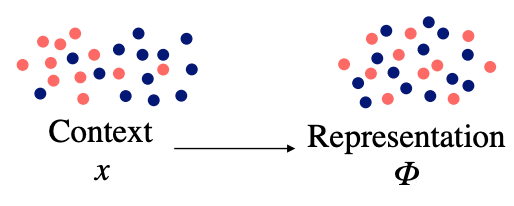
\includegraphics[scale=0.7]{./images/balancing.png}
	\end{frame}

	\begin{frame}{Causal Inference and Domain Adaptation}
		\begin{itemize}
			\item Domain adaptation is a sub-field within machine learning that aims to cope with the situation where the training and the test data fall from different distributions
			\item Domain adaptation aligns the disparity between domains such that the trained model can be generalized into the domain of interest
			\item Johansson et al. (2016) view CI as DA and suggests a objective (loss) function to learn effective representation that well generalizes the trained model in factual domain to counterfactual domain
		\end{itemize}

		% \begin{block}{}
		% 	{\large ``In an election campaign with many competing candidates, a candidate can try to appeal broadly to all voters equally or concentrate more narrowly on winning the support of minorities or special interest groups...
		% 		\vskip5mm
		% 		\textit{Which strategy is better for winning an election?}'' (pg. 856)}
		% \end{block}
	\end{frame}

	\begin{frame}{Problem Setup}
		\begin{itemize}
			\item Binary action set $\mathcal{T}=\{0,1\}$
			\item Causal quantity of interest: $\operatorname{ITE}(x) = Y_{1}(x)-Y_{0}(x)$
			\item Given  $n$ samples $\left\{\left(x_{i}, t_{i}, y_{i}^{F}\right)\right\}_{i=1}^{n}$, where $y_{i}^{F}=$ $t_{i} \cdot Y_{1}\left(x_{i}\right)+\left(1-t_{i}\right) Y_{0}\left(x_{i}\right)$, learn a function $h: \mathcal{X} \times \mathcal{T} \rightarrow \mathcal{Y}$ such that $h\left(x_{i}, t_{i}\right) \approx y_{i}^{F}$
			\item $\hat{\operatorname{ITE}}\left(x_{i}\right)= \begin{cases}y_{i}^{F}-h\left(x_{i}, 1-t_{i}\right), & t_{i}=1 \\ h\left(x_{i}, 1-t_{i}\right)-y_{i}^{F}, & t_{i}=0\end{cases}$
			\item $\hat{P}^{F}=\left\{\left(x_{i}, t_{i}\right)\right\}_{i=1}^{n}$, $\hat{P}^{C F}=\left\{\left(x_{i}, 1-t_{i}\right)\right\}_{i=1}^{n}$
			\item $P^{F}$ and $P^{C F}$ need not to be equal-  the problem of causal inference requires inference over a different
			distribution than the one from which samples are given
			\item In machine learning terms, this means that the feature distribution of the test set differs from that of the train set. This
			is a case of \textit{covariate shift}, which is a special case of domain adaptation.
			% Covariate shift is known to occur in sample selection bias, missing data etc.
			% In this case, missing data for counterfactual directly leads to covariate shift problem. 
		\end{itemize}
	\end{frame}

	\begin{frame}{Balancing Objective}
		\begin{itemize}
			\item Johansson et al. (2016) proposes a method to jointly learns a representation $\Phi: \mathcal{X} \rightarrow$ $\mathbb{R}^{d}$ and $h: \mathbb{R}^{d} \times \mathcal{T} \rightarrow \mathbb{R}$ such that the learned representation minimizes the following objective:
			\begin{align*}
			B_{\mathcal{H}, \alpha, \gamma}(\Phi, h)=&\frac{1}{n} \sum_{i=1}^{n}\left|h\left(\Phi\left(x_{i}\right), t_{i}\right)-y_{i}^{F}\right|\\
			 &+ \alpha \operatorname{disc} \mathcal{H}\left(\hat{P}_{\Phi}^{F}, \hat{P}_{\Phi}^{C F}\right)\\
			 &+\frac{\gamma}{n} \sum_{i=1}^{n}\left|h\left(\Phi\left(x_{i}\right), 1-t_{i}\right)-y_{j(i)}^{F}\right|
			\end{align*}
			\item Let $j(i) \in \arg \min _{j \in\{1 \ldots n\} \text { s.t. } t_{j}=1-t_{i}} \mathrm{~d}\left(x_{j}, x_{i}\right)$ be the nearest neighbor of $x_{i}$ among the group that received
			\item $\operatorname{disc}_{\mathcal{H}}\left(\hat{P}_{\Phi}^{F}, \hat{P}_{\Phi}^{C F}\right) = \underset{{\beta, \beta^{\prime} \in \mathcal{H}}}{\max}\left|\underset{x \sim \hat{P}_{\Phi}^{F}}{\mathbb{E}}\left[L\left(\beta(x), \beta^{\prime}(x)\right)\right]-\underset{x \sim \hat{P}_{\Phi}^{C F}}{\mathbb{E}}\left[L\left(\beta(x), \beta^{\prime}(x)\right)\right]\right|$
			\end{itemize}
			% oftentimes we do feature reweigting and then use those to fit our estimator, this re-weigthing can be understood as special case of representation as well.
			% L is squared loss
	\end{frame}

	\begin{frame}{Components of Objective Function}
		\begin{itemize}
			\item (1) Enabling low-error prediction of the observed outcomes over the factual representation
			\item (2) Make the sampling distributions of factual and counterfactual to be similar
			\item (3) Enabling lowe-rror prediction of unobserved counterfactuals by taking
			into account relevant factual outcomes
			\begin{align}
			B_{\mathcal{H}, \alpha, \gamma}(\Phi, h)=&\frac{1}{n} \sum_{i=1}^{n}\left|h\left(\Phi\left(x_{i}\right), t_{i}\right)-y_{i}^{F}\right|\\
			 &+ \alpha \operatorname{disc} \mathcal{H}\left(\hat{P}_{\Phi}^{F}, \hat{P}_{\Phi}^{C F}\right)\\
			 &+\frac{\gamma}{n} \sum_{i=1}^{n}\left|h\left(\Phi\left(x_{i}\right), 1-t_{i}\right)-y_{j(i)}^{F}\right|
			\end{align}
		\end{itemize}
			% oftentimes we do feature reweigting and then use those to fit our estimator, this re-weigthing can be understood as special case of representation as well.
	\end{frame}

	\begin{frame}{Theoretical Justification of Objective Function}
		\begin{itemize}
			\item $\frac{\lambda}{\mu r}\left(\mathcal{L}_{P^{CF}}\left(\hat{\beta}^{F}(\Phi)\right)-\mathcal{L}_{P^{CF}}\left(\hat{\beta}^{C F}(\Phi)\right)\right)^{2} \leq$
			\begin{align}
			&\min _{h \in \mathcal{H}_{l}} \frac{1}{n} \sum_{i=1}^{n}\left(\left|\hat{y}_{i}^{F}(\Phi, h)-y_{i}^{F}\right|+\left|\hat{y}_{i}^{C F}(\Phi, h)-y_{j(i)}^{F}\right|\right) \\
			&+ \operatorname{disc}_{\mathcal{H}_{l}}\left(\hat{P}_{\Phi}^{F}, \hat{P}_{\Phi}^{C F}\right)  \\
			&+ \frac{K_{0}}{n} \sum_{i: t_{i}=1} \mathrm{~d}_{i, j(i)}+\frac{K_{1}}{n} \sum_{i: t_{i}=0} \mathrm{~d}_{i, j(i)}
			\end{align}
		    \item $\mathcal{H}_{l} \subset \mathbb{R}^{d+1}$ be the space of linear functions
		    \item $\mathcal{L}_{P^{CF}}(\beta)=\mathbb{E}_{(x, t, y) \sim P^{CF}}[L(\beta(x, t), y)]$ be the expected loss of $\beta$ over distribution $P^{CF}$. 
		    \item $\hat{\beta}^{F}(\Phi)=\arg \min _{\beta \in \mathcal{H}_{l}} \mathcal{L}_{\hat{P}_{\Phi}^{F}}(\beta)+\lambda\|\beta\|_{2}^{2}$, $\hat{\beta}^{CF}(\Phi)=\arg \min _{\beta \in \mathcal{H}_{l}} \mathcal{L}_{\hat{P}_{\Phi}^{CF}}(\beta)+\lambda\|\beta\|_{2}^{2}$
		\end{itemize}
			% oftentimes we do feature reweigting and then use those to fit our estimator, this re-weigthing can be understood as special case of representation as well.
			% K0, K1 are lipshitz constant for potentional outcome functions Y0(x), Y1(x) - intuitively it represents the maximum rate of change of continuous function
	\end{frame}

	\begin{frame}{Generalization Bound and Intepretation}
		\begin{itemize}
			\item $\frac{\lambda}{\mu r}\left(\mathcal{L}_{P^{CF}}\left(\hat{\beta}^{F}(\Phi)\right)-\mathcal{L}_{P^{CF}}\left(\hat{\beta}^{C F}(\Phi)\right)\right)^{2} \leq$
			\begin{align}
			&\min _{h \in \mathcal{H}_{l}} \frac{1}{n} \sum_{i=1}^{n}\left(\left|\hat{y}_{i}^{F}(\Phi, h)-y_{i}^{F}\right|+\left|\hat{y}_{i}^{C F}(\Phi, h)-y_{j(i)}^{F}\right|\right) \\
			&+ \operatorname{disc}_{\mathcal{H}_{l}}\left(\hat{P}_{\Phi}^{F}, \hat{P}_{\Phi}^{C F}\right)  \\
			&+ \frac{K_{0}}{n} \sum_{i: t_{i}=1} \mathrm{~d}_{i, j(i)}+\frac{K_{1}}{n} \sum_{i: t_{i}=0} \mathrm{~d}_{i, j(i)}
			\end{align}
			\item Minimizing the bound make the estimator fit on factual distribution to generalize better over counterfactual distribution
			\item It's important to find $\Phi$ such that minimizes the bound
			\item $\Phi$ such that attains low prediction error, less discrepancy between representation space of factual and counterfactual
			\item The GB holds regardless of how $\Phi$ is obtained, e.g. if $\Phi$ is a neural net - it still holds.
		\end{itemize}
			% oftentimes we do feature reweigting and then use those to fit our estimator, this re-weigthing can be understood as special case of representation as well.
			% K0, K1 are lipshitz constant for potentional outcome functions Y0(x), Y1(x) - intuitively it represents the maximum rate of change of continuous function
			% expressive power
	\end{frame}

	\begin{frame}{References}
		\begin{itemize}
			\item Johansson et al., Learning Representations for Counterfactual Inference (2016)
			\item Mansour et al., Domain adaptation: Learning bounds and algorithms (2009)
		\end{itemize}
	\end{frame}


\end{document}

